%\documentclass[a4paper,12pt,twoside]{book}
\documentclass[12pt,times]{report}
\usepackage{mathptmx}%This package supersedes times and mathptm
\usepackage[a4paper,right=2.54cm,left=2.54cm,top=2.54cm,bottom=2.54cm]{geometry}

%%%%paquete para usar citas de diferentes formatos
%%%%%%%%%%%%%%%%%%%%%%%%%%%%%%%%%
%%add al indice
%\usepackage[nottoc,numbib]{tocbibind}
%\usepackage[authoryear,round]{natbib}
\usepackage[utf8]{inputenc}
\usepackage{csquotes}
\usepackage[spanish]{babel}
\usepackage[style=apa ,
%hyperref=auto,
%citestyle=authoryear,
natbib=true,
backend=biber]{biblatex}
\addbibresource{biblio/references.bib}
%\usepackage{biblatex}
%paquete para hiperlinks entre citas e imagenes
%%%%%%%%%%%%%%%%%%%%%%%%%%%%%%%%%
\usepackage[colorlinks=true,
citecolor=blue,
urlcolor=cyan,
bookmarks=true,
linkcolor=blue,
pdftitle={Tesis-nombre-alumno},
pdfauthor={autor nombres}]{hyperref}

\usepackage{amssymb}
\usepackage{graphicx} % for improved inclusion of graphics
%\usepackage{wrapfig} % to include figure with text wrapping around it
\usepackage[margin=10pt,font=small,labelfont=bf]{caption} % for improved layout of figure captions with extra margin, smaller font than text
\usepackage{eucal}
\usepackage[usenames, dvipsnames]{color}
\usepackage[perpage]{footmisc}
%\usepackage[round, sort]{natbib}
\usepackage{ifthen}
\usepackage{multicol} % for pages with multiple text columns, e.g. References
\setlength{\columnsep}{20pt} % space between columns; default 10pt quite narrow
\usepackage[nottoc]{tocbibind} % correct page numbers for bib in TOC, nottoc suppresses an entry for TOC itself
\usepackage{appendix}

%%%----Modificar encabezado y pie de pagina
%%%%%%%%%%%%%%%%%%%%%%%%%%%%%%%%%%%%%%%%%%%%%%%%%%%%%%%%%%%%%%%%%%%%%
\usepackage{fancyhdr} % for better header layout
\newcommand{\changefont}{%
	\fontsize{9pt}{1.5pt}\selectfont
}
\pagestyle{fancy}
\fancyhf{} %% delete default configuration of page
%%\setlength\headheight{15pt}
\fancyhead[L]{\changefont Titulo de tesis aqui}
\fancyhead[R]{\changefont \leftmark}
%%\fancyfoot[L]{\leftmark}
\fancyfoot[R]{\thepage}

%%%%%%%%%%%%%%%%%%%%%%%%%%%%%5
%%%% Configuracion de los parrafos
%\usepackage{setspace}
%\onehalfspacing
%\linespread{1.25} 
\setlength{\parindent}{0.5in} %%sangria
\setlength{\parskip}{3mm}  %%espacio entre parrafos
\linespread{1.3} %This equals 1.5 linespacing in Word
%%%% nuevo parrafo
%%%%%%%%%%%%%%%%%%%%%%%%%%%%%5
%%%% Centrar valores de una tabla
\usepackage{array}
%%CENTRADO HORIZONTAL
\newcolumntype{P}[1]{>{\centering\arraybackslash}p{#1}}
%%CENTRADO VERTICAL
\newcolumntype{M}[1]{>{\centering\arraybackslash}m{#1}}

%%%%%%%%%%%%%%%%%%%%%%%%%%%%%5
%%%%Paquete para alinear texto
\usepackage{ragged2e}
\usepackage{multirow}
\usepackage{makecell}
\usepackage{rotating}
\usepackage{siunitx} % To align the numbers later on
\usepackage[table,xcdraw]{xcolor}
\usepackage{color, colortbl}
\definecolor{Gray}{gray}{0.9}
\definecolor{orange}{rgb}{1,0.647,0}
\definecolor{turq3}{rgb}{0.54, 0.81, 0.94}
\definecolor{turq}{rgb}{0.63, 0.79, 0.95}
\definecolor{bluejean}{rgb}{0.03, 0.27, 0.49}

%%%%%%%%%%%%%%%%%%%%%%%%%
\usepackage{xparse}
\usepackage{expl3}
%%%%funcion de reemplazar regex
\ExplSyntaxOn
\NewDocumentCommand{\replace}{mmm}
{
	\marian_replace:nnn {#1} {#2} {#3}
}

\tl_new:N \l_marian_input_text_tl
\tl_new:N \l_marian_search_tl
\tl_new:N \l_marian_replace_tl

\cs_new_protected:Npn \marian_replace:nnn #1 #2 #3
{
	\tl_set:Nn \l_marian_input_text_tl { #1 }
	\tl_set:Nn \l_marian_search_tl { #2 }
	\tl_set:Nn \l_marian_replace_tl { #3 }
	\regex_replace_all:nnN { \b\u{l_marian_search_tl}\b } { \u{l_marian_replace_tl} } \l_marian_input_text_tl
	\tl_use:N \l_marian_input_text_tl
}
\ExplSyntaxOff

%%%%%%%%%%%%%%%%%%%%%%%%%%%%%%%%%%%%%%
\usepackage{amsmath}
\numberwithin{equation}{chapter} %%enumerar ecuaciones
\renewcommand{\theequation}{Ecuación \thechapter.\arabic{equation}}   
\usepackage{mathtools, nccmath, cool}
%%%Configuraciones de biblatex

%%%hel
%%%%\citeauthor
\makeatletter

%%%%%%%%%%%%
\DeclareCiteCommand{\citeauthor}
{\boolfalse{citetracker}%
	\boolfalse{pagetracker}%
	\usebibmacro{prenote}}
{\ifciteindex
	{\indexnames{labelname}}
	{}%
	\printtext[bibhyperref]{\printnames{labelname}}}
{\multicitedelim}
{\usebibmacro{postnote}}


\DeclareCiteCommand{\citetitle}
{\boolfalse{citetracker}%
	\boolfalse{pagetracker}%
	\usebibmacro{prenote}}
{\ifciteindex
	{\indexfield{indextitle}}
	{}%
	\printtext[bibhyperref]{\printfield[citetitle]{labeltitle}}}
{\multicitedelim}
{\usebibmacro{postnote}}

\DeclareCiteCommand{\cite}
{\usebibmacro{prenote}}
{\usebibmacro{citeindex}%
	\printtext[bibhyperref]{\usebibmacro{cite}}}
{\multicitedelim}
{\usebibmacro{postnote}}

\DeclareCiteCommand*{\cite}
{\usebibmacro{prenote}}
{\usebibmacro{citeindex}%
	\printtext[bibhyperref]{\usebibmacro{citeyear}}}
{\multicitedelim}
{\usebibmacro{postnote}}

\DeclareCiteCommand{\parencite}[\mkbibparens]
{\usebibmacro{prenote}}
{\usebibmacro{citeindex}%
	\printtext[bibhyperref]{\usebibmacro{cite}}}
{\multicitedelim}
{\usebibmacro{postnote}}

\DeclareCiteCommand*{\parencite}[\mkbibparens]
{\usebibmacro{prenote}}
{\usebibmacro{citeindex}%
	\printtext[bibhyperref]{\usebibmacro{citeyear}}}
{\multicitedelim}
{\usebibmacro{postnote}}

\DeclareCiteCommand{\footcite}[\mkbibfootnote]
{\usebibmacro{prenote}}
{\usebibmacro{citeindex}%
	\printtext[bibhyperref]{ \usebibmacro{cite}}}
{\multicitedelim}
{\usebibmacro{postnote}}

\DeclareCiteCommand{\footcitetext}[\mkbibfootnotetext]
{\usebibmacro{prenote}}
{\usebibmacro{citeindex}%
	\printtext[bibhyperref]{\usebibmacro{cite}}}
{\multicitedelim}
{\usebibmacro{postnote}}

\DeclareCiteCommand{\textcite}
{\boolfalse{cbx:parens}}
{\usebibmacro{citeindex}%
	\printtext[bibhyperref]{\usebibmacro{textcite}}}
{\ifbool{cbx:parens}
	{\bibcloseparen\global\boolfalse{cbx:parens}}
	{}%
	\multicitedelim}
{\usebibmacro{textcite:postnote}}
\makeatother
\makeatletter
\let\abx@macro@citeOrig\abx@macro@cite
\renewbibmacro{cite}{%
	\bibhyperref{%
		\let\bibhyperref\relax\relax%
		\abx@macro@citeOrig%
	}%
}
\let\abx@macro@textciteOrig\abx@macro@textcite
\renewbibmacro{textcite}{%
	\bibhyperref{%
		\let\bibhyperref\relax\relax%
		\abx@macro@textciteOrig%
	}%
}%

\makeatother

%%%%%%%%%%%%%%%%%%%%%%%%%%%%%%%%%%%%%%%%%%%
\begin{document}

\begin{titlepage}

	\begin{center}
		%%%cargar imagen
	    
\includegraphics[width=0.45\textwidth]{images_repo/esanlogomin}
		\vspace*{2cm} \\
		UNIVERSIDAD ESAN \vspace*{1ex} \\
		FACULTAD DE INGENIERÍA \vspace*{1ex} \\
		INGENIERÍA DE TECNOLOGÍAS DE INFORMACIÓN Y SISTEMAS\vspace*{8ex} \\
		\textbf{Implementación de un modelo de Deep Learning para la traducción de lenguaje de señas para personas con discapacidades del habla}
		\vspace*{8ex}\\	
		
		Adrian Gómez Sánchez Bendezú AA\\
		Asesor: Marks Calderón		
		\vfill
		
		Lima, \today 
		
	\end{center}
\end{titlepage}
%%cambiar nombres de objetos para el indice y otros
\renewcommand{\listfigurename}{Índice de Figuras}
\renewcommand{\tablename}{Tabla}
\renewcommand{\listtablename}{Índice de Tablas}

\thispagestyle{plain}
\begin{center}
	\vspace*{1.5cm}
	{\Large \bfseries  Resumen}
\end{center}
\vspace{0.5cm}
Lorem ipsum dolor sit amet, consectetur adipiscing elit, sed do eiusmod tempor incididunt ut labore et dolore magna aliqua. Ac odio tempor orci dapibus ultrices in iaculis nunc sed. Vivamus arcu felis bibendum ut tristique et egestas quis ipsum. Odio morbi quis commodo odio aenean sed adipiscing diam donec. Donec ultrices tincidunt arcu non sodales neque sodales ut. Fusce ut placerat orci nulla pellentesque dignissim enim sit amet. Facilisi etiam dignissim diam quis enim lobortis. Sit amet justo donec enim diam vulputate ut pharetra. Gravida in fermentum et sollicitudin ac orci phasellus egestas. Ultricies tristique nulla aliquet enim tortor at auctor. Nullam vehicula ipsum a arcu cursus vitae congue mauris. Convallis posuere morbi leo urna molestie at elementum eu facilisis. Elit at imperdiet dui accumsan sit amet nulla. Amet consectetur adipiscing elit pellentesque habitant morbi tristique senectus et. Mauris in aliquam sem fringilla ut morbi. Ultricies integer quis auctor elit sed vulputate mi sit. Nulla pellentesque dignissim enim sit amet venenatis urna cursus eget. Ac feugiat sed lectus vestibulum mattis ullamcorper. Eu augue ut lectus arcu bibendum. Rhoncus dolor purus non enim praesent elementum. 

Nulla facilisi cras fermentum odio eu feugiat pretium. Massa massa ultricies mi quis hendrerit. Id leo in vitae turpis massa sed elementum. Quis vel eros donec ac odio tempor orci. Netus et malesuada fames ac turpis egestas integer eget aliquet. Velit ut tortor pretium viverra suspendisse potenti. Ut enim blandit volutpat maecenas. Nibh tellus molestie nunc non blandit. Mus mauris vitae ultricies leo integer malesuada nunc vel. Vel elit scelerisque mauris pellentesque pulvinar pellentesque habitant. Neque viverra justo nec ultrices dui sapien eget. Vitae aliquet nec ullamcorper sit. Dui id ornare arcu odio ut sem nulla pharetra diam. Et magnis dis parturient montes. Varius morbi enim nunc faucibus.
\newline

\textbf{Palabras claves: } uno, dos, tres, cuatro
\thispagestyle{plain}
\begin{center}
	\vspace*{1.5cm}
	{\Large \bfseries  Abstract}
\end{center}
\vspace{0.5cm}
Lorem ipsum dolor sit amet, consectetur adipiscing elit, sed do eiusmod tempor incididunt ut labore et dolore magna aliqua. Ac odio tempor orci dapibus ultrices in iaculis nunc sed. Vivamus arcu felis bibendum ut tristique et egestas quis ipsum. Odio morbi quis commodo odio aenean sed adipiscing diam donec. Donec ultrices tincidunt arcu non sodales neque sodales ut. Fusce ut placerat orci nulla pellentesque dignissim enim sit amet. Facilisi etiam dignissim diam quis enim lobortis. Sit amet justo donec enim diam vulputate ut pharetra. Gravida in fermentum et sollicitudin ac orci phasellus egestas. Ultricies tristique nulla aliquet enim tortor at auctor. Nullam vehicula ipsum a arcu cursus vitae congue mauris. Convallis posuere morbi leo urna molestie at elementum eu facilisis. Elit at imperdiet dui accumsan sit amet nulla. Amet consectetur adipiscing elit pellentesque habitant morbi tristique senectus et. Mauris in aliquam sem fringilla ut morbi. Ultricies integer quis auctor elit sed vulputate mi sit. Nulla pellentesque dignissim enim sit amet venenatis urna cursus eget. Ac feugiat sed lectus vestibulum mattis ullamcorper. Eu augue ut lectus arcu bibendum. Rhoncus dolor purus non enim praesent elementum. 

Nulla facilisi cras fermentum odio eu feugiat pretium. Massa massa ultricies mi quis hendrerit. Id leo in vitae turpis massa sed elementum. Quis vel eros donec ac odio tempor orci. Netus et malesuada fames ac turpis egestas integer eget aliquet. Velit ut tortor pretium viverra suspendisse potenti. Ut enim blandit volutpat maecenas. Nibh tellus molestie nunc non blandit. Mus mauris vitae ultricies leo integer malesuada nunc vel. Vel elit scelerisque mauris pellentesque pulvinar pellentesque habitant. Neque viverra justo nec ultrices dui sapien eget. Vitae aliquet nec ullamcorper sit. Dui id ornare arcu odio ut sem nulla pharetra diam. Et magnis dis parturient montes. Varius morbi enim nunc faucibus.
\newline

\textbf{Keywords: } uno, dos, tres, cuatro
\thispagestyle{plain}
\begin{center}
	\vspace*{1.5cm}
	{\Large Para mi X, Y,X}
\end{center}


\thispagestyle{plain}
\begin{center}
	\vspace*{1.5cm}
	{\Large \bfseries  Agradecimientos}
\end{center}
\vspace{0.5cm}
Lorem ipsum dolor sit amet, consectetur adipiscing elit, sed do eiusmod tempor incididunt ut labore et dolore magna aliqua. Ac odio tempor orci dapibus ultrices in iaculis nunc sed. Vivamus arcu felis bibendum ut tristique et egestas quis ipsum. Odio morbi quis commodo odio aenean sed adipiscing diam donec. Donec ultrices tincidunt arcu non sodales neque sodales ut. Fusce ut placerat orci nulla pellentesque dignissim enim sit amet. Facilisi etiam dignissim diam quis enim lobortis. Sit amet justo donec enim diam vulputate ut pharetra. Gravida in fermentum et sollicitudin ac orci phasellus egestas. Ultricies tristique nulla aliquet enim tortor at auctor. Nullam vehicula ipsum a arcu cursus vitae congue mauris. Convallis posuere morbi leo urna molestie at elementum eu facilisis. Elit at imperdiet dui accumsan sit amet nulla. Amet consectetur adipiscing elit pellentesque habitant morbi tristique senectus et. Mauris in aliquam sem fringilla ut morbi. Ultricies integer quis auctor elit sed vulputate mi sit. Nulla pellentesque dignissim enim sit amet venenatis urna cursus eget. Ac feugiat sed lectus vestibulum mattis ullamcorper. Eu augue ut lectus arcu bibendum. Rhoncus dolor purus non enim praesent elementum. 

Nulla facilisi cras fermentum odio eu feugiat pretium. Massa massa ultricies mi quis hendrerit. Id leo in vitae turpis massa sed elementum. Quis vel eros donec ac odio tempor orci. Netus et malesuada fames ac turpis egestas integer eget aliquet. Velit ut tortor pretium viverra suspendisse potenti. Ut enim blandit volutpat maecenas. Nibh tellus molestie nunc non blandit. Mus mauris vitae ultricies leo integer malesuada nunc vel. Vel elit scelerisque mauris pellentesque pulvinar pellentesque habitant. Neque viverra justo nec ultrices dui sapien eget. Vitae aliquet nec ullamcorper sit. Dui id ornare arcu odio ut sem nulla pharetra diam. Et magnis dis parturient montes. Varius morbi enim nunc faucibus.
\newline



% outline
\tableofcontents            % print the table of contents

%: ----------------------- contents ------------------------

\setcounter{secnumdepth}{3} % organisational level that receives a numbers
\setcounter{tocdepth}{3}    % print table of contents for level 3

% levels are: 0 - chapter, 1 - section, 2 - subsection, 3 - subsection


%: ----------------------- list of figures/tables ------------------------

\listoffigures	% print list of figures

\listoftables  % print list of tables



\chapter{PLANTEAMIENTO DEL PROBLEMA}
\section{Descripción de la Realidad Problemática}

Las discapacidades del habla abarcan una amplia gama de condiciones que afectan la capacidad de una persona para comunicarse verbalmente de manera clara y fluida. Según la American Speech-Language-Hearing Association (ASHA), las discapacidades del habla pueden originarse por una variedad de razones, que van desde dificultades físicas en los órganos responsables de la producción del habla, hasta trastornos neurológicos que impactan la habilidad de hablar de manera clara y fluida.

Para las personas con discapacidades del habla, el lenguaje de señas se convierte en una herramienta invaluable que les permite expresar sus pensamientos, emociones y necesidades de manera efectiva. El lenguaje de señas es un sistema de comunicación visual y gestual utilizado por personas sordas o con discapacidades auditivas para comunicarse entre sí y con personas que pueden escuchar.

La Organización Mundial de la Salud afirmó que aproximadamente 70 millones de personas en el mundo son sordomudas. Un total de 360 millones de personas son sordas, y 32 millones de ellas son niños. Sin embargo, en Perú, de acuerdo con los resultados del Censo de Población y Vivienda 2017, como se puede observar en la Figura \ref{1:fig 1}, hay un elevado porcentaje de personas que tienen dificultades para oír y para hablar o comunicarse.

El INEI también afirma que las personas presentan estas capacidades utilizan como apoyo para comunicarse su voz (19,8\% ), gesto y manos (11,9\% ) y lenguaje de señas (2,9\% ). Y debido a estas dificultades, estas personas se ven afectadas en el ámbito social y también laboral, por no poder expresarse debido a sus discapacidades. Según la Organización Mundial de Salud, las personas con estas discapacidades tienen más probabilidades de experimentar pobreza y exclusión social, y tienen menos probabilidades de tener un empleo remunerado que las personas sin discapacidades. En base a encuestas realizadas por la organización Incluyeme, alrededor del 72\% de personas con discapacidad se encuentra desempleado, como se puede observar en la Figura \ref{1:fig 2}.

El objetivo principal de esta investigación es lograr un aumento significativo en la comunicación entre personas con discapacidades del habla y aquellas que no las tienen, a través de la implementación de un modelo de traducción de lenguaje de señas utilizando Deep Learning. Este modelo busca facilitar una interacción más fluida y efectiva, permitiendo a las personas con discapacidades del habla expresar sus pensamientos, emociones y necesidades de manera más accesible y comprensible para quienes no conocen el lenguaje de señas.

\begin{figure}[h]
	\begin{center}
		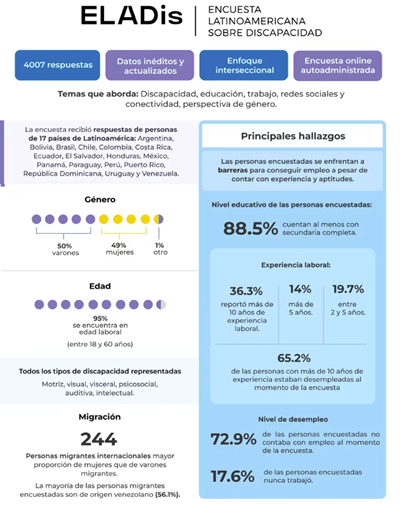
\includegraphics[width=0.5\textwidth]{1/figures/Encuesta_personas_discapacidad.png}
		\caption{Encuesta de personas con discapacidad . Fuente: \cite{encuesta_personas_discapacidad}}
		\label{1:fig 2}
	\end{center}
\end{figure}

\begin{figure}[h]
	\begin{center}
		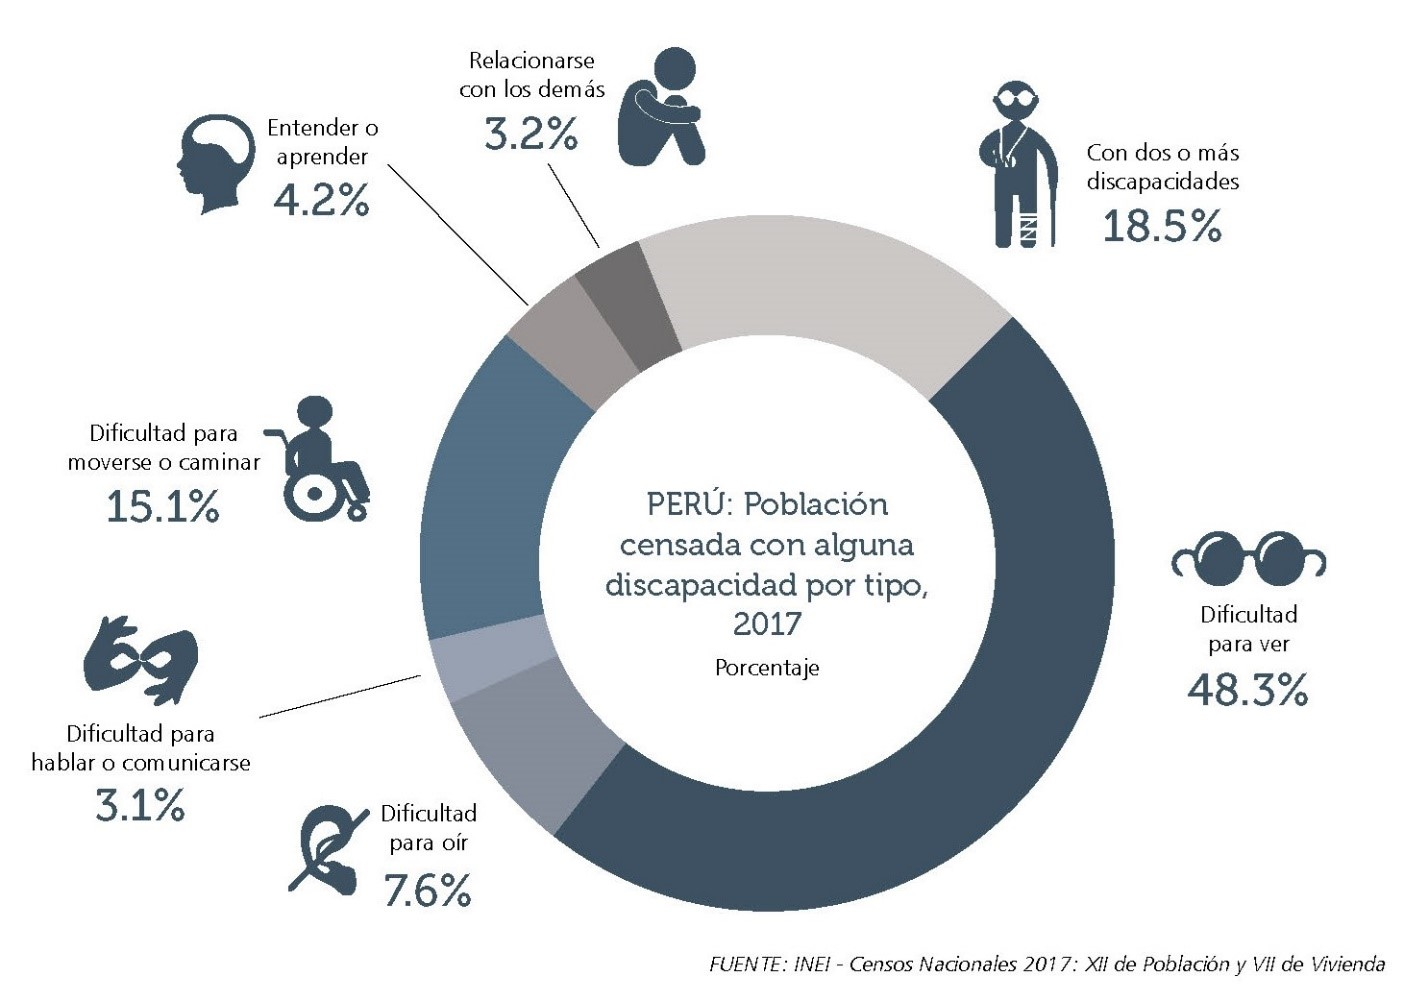
\includegraphics[width=0.5\textwidth]{1/figures/personas_discapacidad.jpg}
		\caption{\% de personas con discapacidad. Fuente: \cite{porcentaje de_personas_discapacidad}}
		\label{1:fig 1}
	\end{center}
\end{figure}




\section{Formulación del Problema}


\subsection{Problema General}
\newcommand{\ProblemaGeneral}{
	El problema general de esta investigación es la Dificultad de comunicación para personas con indiscapacidades del habla al interactuar con personas que no conocen el lenguaje de señas.
}
\ProblemaGeneral
\subsection{Problemas Espec\'{i}ficos}
\newcommand{\Pbone}{
¿Cómo pueden los modelos de Deep Learning leer e interpretar el lenguaje de señas?
}
\newcommand{\Pbtwo}{
¿Cómo los modelos de Deep Learning pueden predecir lenguaje de señas para una conversación fluida entre una persona con discacidad y otra sin ninguna?
}
\newcommand{\Pbthree}{
¿De que manera los modelos Deep Learning pueden  diferenciar entre los distintos tipos de lenguajes de señas?
}

\begin{itemize}
	\item \Pbone
	\item \Pbtwo
	\item \Pbthree
\end{itemize}

\section{Objetivos de la Investigación}
\subsection{Objetivo General}
\newcommand{\ObjetivoGeneral}{
Mediante el modelo de Deep Learning se utilizará una herramienta de traducción entre personas con discapacidades del habla que utilizan lenguaje de señas con personas que no conocen este lenguaje. 
}
\ObjetivoGeneral
\subsection{Objetivos Espec\'{i}ficos}
\newcommand{\Objone}{
Traducir lenguajes de señas utilizando técnicas de visión de computadora y el uso de Redes Neuronales.
}
\newcommand{\Objtwo}{
El modelo puede ser entrenado utilizando conjuntos extensos de datos para mejorar su exactitud y capacidad de interpretación de gestos. Esto facilita una comunicación más natural y sin interrupciones entre individuos con y sin discapacidad auditiva.
}
\newcommand{\Objthree}{
Los modelos de Deep Learning pueden entrenarse con conjuntos de datos etiquetados que contienen ejemplos de diferentes lenguajes de señas. Esto les permite aprender a asociar patrones visuales específicos con cada lenguaje de señas.
}

\begin{itemize}
	\item {\Objone}
	\item {\Objtwo}
	\item {\Objthree}
\end{itemize}

\section{Justificación de la Investigación}

\subsection{Teórica}
Esta investigación se realiza 

\subsection{Práctica}
Al culminar la investigación 

\subsection{Metodológica}. 

\section{Delimitación del Estudio}

\subsection{Espacial}
Para la presente investigación 

\subsection{Temporal}
Los datos que serán necesari. 

\subsection{Conceptual}
Esta investigación se 

\section{Hipótesis}

\subsection{Hipótesis General}
\newcommand{\HipotesisGeneral}{
El uso de técnicas de.
}
\HipotesisGeneral
\subsection{Hipótesis Específicas}
\newcommand{\Hone}{
	x
}
\newcommand{\Htwo}{
	y
}
\newcommand{\Hthree}{
	z	
}
\newcommand{\Hfour}{
	cv
}
\newcommand{\Hfive}{
	xws
}
\begin{itemize}
	\item \Hone
	\item \Htwo
	\item \Hthree
	\item \Hfour
	\item \Hfive
\end{itemize}

\subsection{Matriz de Consistencia}
A continuación se presenta la matriz de consistencia elaborada para la presente investigación (véase Anexo \ref{1:table}).


\chapter{MARCO TEÓRICO}
\section{Antecedentes de la investigación}
En esta sección se presentarán diversos artículos de investigación o tesis las cuales abordarán diversas técnicas y enfoques que se emplearon para afrontar problemas similares al de esta tesis. Asimismo, a continuación se presenta un cuadro resumen (véase Anexo \ref{A:table}) de lo que se presenta en esta sección.


\subsection{DeepASL: Enabling Ubiquitous and Non-IntrusiveWord and Sentence-Level Sign Language Translation}

DeepASL es un modelo de traducción de lenguaje de señas basada en Deep Learning que permite la traducción de ASL (American Sign Language) tanto a nivel de palabra como de oración de manera no intrusiva, es decir  este método no requiere que el usuario use algún equipo que cambie su comportamiento natural. Utiliza una luz infrarroja y un innovador sistema jerárquico bidireccional de redes neuronales recurrentes (HB-RNN) junto con un marco probabilístico basado en la Clasificación Temporal Conexionista (CTC).

\subsubsection {Metodología}
La metodología del documento incluye varias etapas, a partir de la recolección de datos hasta la implementación del modelo. A continuación, se presenta un resumen de la metodología junto con gráficos relevantes:

\begin{enumerate}
	\item {Recolección de datos: }
	Se recolectaron 7,306 muestras de 11 participantes, de las cuales 56 palabras y 100 oraciones comúnmente usadas en lenguaje de señas americano. También se recolectaron 1,178 muestras bajo diferentes condiciones de iluminación, posturas corporales e interferencia en la escena para evaluar la robustez del sistema.
	\item {Captura de Señales: }
	Se utilizó el dispositivo Leap Motion, que emplea luz infrarroja para capturar de manera no intrusiva las señas de ASL. Leap Motion extrae la información de las articulaciones del esqueleto de los dedos, palmas y antebrazos.
	\item {Extracción de Características}
	Se aprovecharon conocimientos del dominio de ASL para extraer las características clave de las señas, incluyendo la forma de la mano, el movimiento de la mano y la ubicación relativa de las dos manos.
	\item {Modelado y Traducción: }
	Se empleó un sistema jerárquico bidireccional de redes neuronales recurrentes (HB-RNN) para modelar la estructura espacial y dinámica temporal de las características extraídas para la traducción a nivel de palabra. Para la traducción a nivel de oración, se adoptó un marco probabilístico basado en la Clasificación Temporal Conexionista (CTC).
	\item {Evaluación del Rendimiento: }
	Se evaluó el rendimiento del sistema en términos de precisión de traducción, robustez bajo diferentes condiciones del mundo real y rendimiento del sistema (tiempo de ejecución, uso de memoria y consumo de energía). DeepASL se implementó en tres plataformas con diferente poder de cómputo: una computadora de escritorio, una plataforma móvil Nvidia Jetson TX1 y una tableta Microsoft Surface Pro 4.
\end{enumerate}
\subsubsection {Conclusiones}
El modelo DeepASL demostró ser robusto en diversas condiciones de iluminación, posturas corporales y con diferentes fuentes de interferencia.
El sistema mostró un rendimiento de tiempo de ejecución de 282ms en el peor de los casos y fue capaz de soportar un número suficiente de inferencias para su uso diario en plataformas móviles y de tabletas.


\subsection{Sign Language Fingerspelling Recognition Using DepthInformation and Deep Belief Networks}
Este sistema traductor de lenguaje de señas contiene una técnica de profundidad utilizando redes de creencias profundas (DBNs) para la detección de dedos en el deletreo del lenguaje de señas. Se utilizan momentos de Zernike y histogramas de gradientes orientados (HOG) como características discriminativas.

\subsubsection {Metodología}

\begin{enumerate}
	\item {Preprocesamiento de Datos: }
	Se capturan secuencias de imágenes que representan la dinámica de las señas. Las imágenes son normalizadas y redimensionadas para mantener la consistencia en los datos de entrada.
	\item {Modelo Híbrido CNN-RNN: }
	La CNN se utiliza para extraer características espaciales de cada imagen en la secuencia. Una RNN, específicamente una LSTM, se emplea para capturar dependencias temporales entre las secuencias de imágenes. El modelo híbrido es entrenado con un conjunto de datos etiquetado, ajustando hiperparámetros para optimizar el rendimiento.
	\item {Evaluación del Modelo: }
	En este modelo de traducción, para medir los resultados se enfocan en las métricas de precisión, sensibilidad, especificidad y F1-score. Se realizan pruebas para evaluar la robustez del modelo ante variaciones en las condiciones de iluminación y ángulos de captura.
\end{enumerate}
\subsubsection {Conclusiones: }
	La combinación de CNN y RNN mejora significativamente el reconocimiento de señas al capturar tanto características espaciales como temporales. Se identifican desafíos como la necesidad de más datos para entrenar adecuadamente el modelo y la importancia de la diversidad en el conjunto de datos. Futuras investigaciones pueden enfocarse en mejorar la eficiencia computacional del modelo y explorar otras arquitecturas híbridas.


\subsection{Deep learning-based sign language recognition system for static signs }
	El documento describe un estudio sobre el reconocimiento de letras del alfabeto manual utilizando información de profundidad y redes de creencias profundas (DBN). El objetivo principal es mejorar la precisión y eficiencia del reconocimiento de lenguaje de señas, específicamente el dactilológico.

\subsubsection {Metodología: }
	\begin{enumerate}
		\item {Adquisición de Datos: }
			Se utilizaron sensores de profundidad para capturar imágenes de las manos formando las letras del alfabeto manual. Los datos capturados incluyen tanto imágenes de profundidad como información adicional relevante para el reconocimiento de señas.
		
		\item {Preprocesamiento de Datos: }
			Las imágenes de profundidad se preprocesaron para resaltar las características importantes y reducir el ruido. Se aplicaron técnicas de normalización y segmentación para preparar los datos para su uso en el modelo de aprendizaje profundo.
			
		\item {Modelo de Aprendizaje: }
			Se utilizó una Red de Creencias Profundas (DBN) para el reconocimiento de letras. El modelo se entrenó utilizando los datos preprocesados, ajustando los parámetros para optimizar el rendimiento.
			
		\item {Validación y Evaluación: }
			Se dividieron los datos en conjuntos de entrenamiento y prueba. Se utilizaron métricas de precisión, recall y F1-score para evaluar el rendimiento del modelo. Se realizaron pruebas cruzadas para asegurar la robustez del modelo.
			
\end{enumerate}
\subsubsection {Conclusiones: }
	El uso de información de profundidad en combinación con DBN es una técnica efectiva para el reconocimiento de lenguaje de señas. La metodología propuesta puede ser utilizada para desarrollar sistemas de traducción de lenguaje de señas más eficientes y precisos. Se identificaron áreas para futuras investigaciones, como la inclusión de más datos y la optimización de los modelos para diferentes lenguas de señas.
	

\subsection{Enabling Real-time Sign Language Translation on Mobile Platforms with On-board Depth Cameras}
Este trabajo presenta un sistema para la traducción de lenguaje de señas en tiempo real utilizando cámaras de profundidad en dispositivos móviles. El sistema, denominado SUGO, utiliza un modelo de red neuronal convolucional 3D (3DCNN) basado en ResNet-18, adaptado para la extracción de características de secuencias de imágenes en video.
\subsubsection {Metodología: }
	\begin{enumerate}
		\item {Arquitectura del modelo: }
		 Se utiliza el modelo ResNet-18 adaptado a 3DCNN, preentrenado con el dataset Kinetics-400 y luego reentrenado con un dataset propio.
		\item {Limpieza y cuantización: }
		Para reducir el tamaño del modelo y su complejidad computacional, se aplican técnicas de poda de filtros y cuantificación de pesos, convirtiendo todos los parámetros de peso a unidades de punto flotante de menor precisión.
		\item {Aumento de base de datos: }
		Se genera un dataset aumentado para hacer el modelo más robusto frente a ruidos de movimiento. Este dataset incluye datos que imitan los ruidos de movimiento que pueden introducirse en escenarios de uso real.
		\item {Segmentación de palabras: }
		Se implementa un módulo de segmentación de palabras que utiliza una ventana deslizante para dividir secuencias de video en subconjuntos manejables para la clasificación de palabras individuales.
	\end{enumerate}
\subsubsection {Conclusiones: }
La poda de filtros y la cuantificación de pesos reducen el tamaño y la complejidad del modelo, haciéndolo adecuado para su operación en dispositivos móviles con recursos limitados. La adición de datos aumentados durante la fase de entrenamiento mejora la resiliencia del sistema frente a ruidos de movimiento, aunque introduce una ligera degradación (0.3\%). El sistema demuestra una capacidad efectiva para clasificar gestos de lenguaje de señas en tiempo real en diversas condiciones de iluminación y movimiento.


\subsection{Using Deep Learning in Sign Language Translation to Text}
El documento revisa múltiples estudios sobre el reconocimiento de lenguaje de señas utilizando técnicas de aprendizaje profundo y captura de movimiento. Se enfoca en diferentes lenguajes de señas y diversas metodologías aplicadas, como redes neuronales convolucionales (CNN), redes neuronales de creencias profundas (DBN), y otras técnicas avanzadas de aprendizaje automático. El objetivo principal es analizar y comparar estas metodologías para entender sus fortalezas y limitaciones en el contexto del reconocimiento de lenguaje de señas.
\subsubsection {Metodología: }
	\begin{enumerate}
		\item {Redes Neuronales Convolucionales (CNN): }
		Estas redes son eficaces en la extracción de características espaciales de las imágenes, lo que las hace adecuadas para el reconocimiento de gestos y señas.
		\item {Redes de Creencias Profundas (DBN): }
		Utilizadas para la extracción de características de datos de profundidad, lo que ayuda en la identificación precisa de las formas y movimientos de las manos.
		\item {Clasificación Temporal Conexista (CTC): }
		Una técnica que permite el reconocimiento de secuencias sin necesidad de segmentación explícita de los datos de entrada.
		\item {Cámaras de Profundidad a Bordo: }
		Utilizadas para capturar datos en 3D, proporcionando información detallada sobre la posición y el movimiento de las manos.
	\end{enumerate}
\subsubsection {Conclusiones: }
Los estudios revisados muestran una alta variabilidad en la precisión y efectividad de las técnicas utilizadas, dependiendo del lenguaje de señas y la complejidad de los gestos. Este estudio utilizó CNN y cámaras de profundidad y lograron una precisión superior al 90\% en el reconocimiento de ciertos lenguajes de señas, como el American Sign Language (ASL). Las técnicas enfrentan dificultades cuando se trata de señas complejas o cuando el modelo debe generalizar a diferentes personas y contextos. La disponibilidad y calidad de los datos de entrenamiento son cruciales para el rendimiento de los modelos de aprendizaje profundo. Estudios con grandes conjuntos de datos de alta calidad obtuvieron mejores resultados.



\section{Bases Teóricas}
\subsection{Machine Learning}
 Es un subcampo de l]ecutar dificultosos procesos aprendiendo de datos, en lugar de seguir reglas preprogramadas \parencite{tec_royal2017machine}.

 es importante mencionar que existen también cinco tipos de problemas de aprendizaje que se pueden enfrentar: regresión, clasificación, simulación, optimización y clusterización \parencite{bk_gollapudi2016practical}. Por otro lado, el aprendizaje automático también posee una división por subcampos que se puede observar en la Figura 14.
%%Figura
 \subsection{Natural Language Processing (NLP)}
 Naturalmano \parencite{bk_goyal2018deep}. Otra definición para este término implica que es un campo especializado de la informática que es

 De acuerdo con \citet{bk_goyal2018deep}, e
 

\section{Marco Conceptual}
Para de


\chapter{METODOLOGÍA DE LA INVESTIGACIÓN}
\section{Diseño de la investigación}
En esta sección del documento se explicará cual es el diseño, el tipo y el enfoque del trabajo de
investigación, así como también la población y la muestra. 
%Para finalizar se explicará el
%proceso de aplicación de las redes neuronales convolucionales.
\subsection{Diseño no experimental}
El diseño es no experimental longitudinal, ya que las variables no serán manipuladas y serán analizadas tal como se encuentran. Es decir, tanto los datos textuales (noticias) y el precio del cobre serán analizados sin ningún cambio aplicando técnicas de procesamiento de lenguaje natural y algoritmos de aprendizaje automático con la finalidad de crear un modelo productivo robusto y facilitar la predicción del cobre. Asimismo, la recolección de datos que se realizará será en un determinado periodo de tiempo. 

\subsection{Tipo explicativo}
El alcance de la presente investigación es explicativo debido a que se busca explicar el comportamiento volátil del precio del cobre en base a noticias de periódicos digitales y además predecirlo.

\subsection{Enfoque cuantitativo}
El enfoque esta investigación es cuantitativo dado que se empleará técnicas del procesamiento de lenguaje natural (NLP), las cuales conllevan a procesar los datos de tipo textual a numéricos (vectores de características) y con ello posteriormente usar técnicas estadísticas como la regresión lineal para la predicción del precio del cobre.



\section{Población y muestra}

 Nisi porta lorem mollis aliquam ut porttitor leo. Aenean pharetra magna ac placerat vestibulum. Est placerat in egestas erat imperdiet sed euismod. Velit euismod in pellentesque massa placerat. Enim praesent elementum facilisis leo vel fringilla. Ante in nibh mauris cursus mattis molestie a iaculis. Erat pellentesque adipiscing commodo elit at imperdiet dui accumsan sit. Porttitor lacus luctus accumsan tortor posuere ac ut. Tortor at auctor urna nunc id. A iaculis at erat pellentesque adipiscing commodo elit. La Figura \ref{fig1} y el Cuadro \ref{tab:widgets}

	\begin{figure}[h]
		\begin{center}
			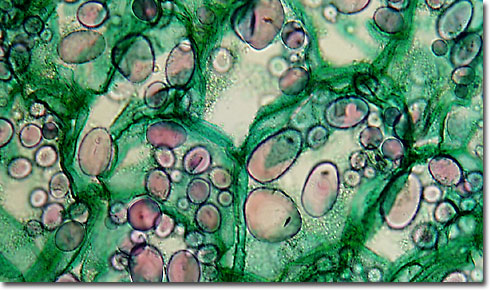
\includegraphics[width=0.8\textwidth]{3/figures/largepotato.jpg}
			\caption{Prueba de Figura}
			\label{fig1}
		\end{center}
		
	\end{figure}


\section{Operacionalización de Variables}

Nisi porta lorem mollis aliquam ut porttitor leo. Aenean pharetra magna ac placerat vestibulum. Est placerat in egestas erat imperdiet sed euismod. Velit euismod in pellentesque massa placerat. Enim praesent elementum facilisis leo vel fringilla. Ante in nibh mauris cursus mattis molestie a iaculis. Erat pellentesque adipiscing commodo elit at imperdiet dui accumsan sit. Porttitor lacus luctus accumsan tortor posuere ac ut. Tortor at auctor urna nunc id. A iaculis at erat pellentesque adipiscing commodo elit.
\section{Instrumentos de medida}
Nisi porta lorem mollis aliquam ut porttitor leo. Aenean pharetra magna ac placerat \begin{itemize}
	\item muscle and fat cells remove glucose from the blood,
	\item cells breakdown glucose via glycolysis and the citrate cycle, storing its energy in the form of ATP,
	\item liver and muscle store glucose as glycogen as a short-term energy reserve,
	\item adipose tissue stores glucose as fat for long-term energy reserve, and
	\item cells use glucose for protein synthesis.
\end{itemize}

\section{Técnicas de recolección de datos}
Nisi porta lorem mollis aliquam ut porttitor leo. Aenean pharetra magna ac placerat vestibulum. Est placerat in egestas erat imperdiet sed euismod. Velit euismod in pellentesque massa placerat. Enim praesent elementum facilisis leo vel fringilla. Ante in nibh mauris cursus mattis molestie a iaculis. Erat pellentesque adipiscing commodo elit at imperdiet dui accumsan sit. Porttitor lacus luctus accumsan tortor posuere ac ut. Tortor at auctor urna nunc id. A iaculis at erat pellentesque adipiscing commodo elit.

\LaTeX{} is great at typesetting mathematics. Let $X_1, X_2, \ldots, X_n$ be a sequence of independent and identically distributed random variables with
\begin{equation}
	S_n = \frac{X_1 + X_2 + \cdots + X_n}{n}
	= \frac{1}{n}\sum_{i}^{n} X_i
	\label{eq1}
\end{equation}

La Ecuación \ref{eq1} denote their mean. Then as $n$ approaches infinity, the random variables $$\sqrt{n}(S_n - \mu)$$ converge in distribution to a normal $\mathcal{N}(0, \sigma^2)$.

\section{Técnicas para el procesamiento y análisis de la información}
Nisi porta lorem mollis aliquam ut porttitor leo. Aenean pharetra magna ac placerat vestibulum. Est placerat in egestas erat imperdiet sed euismod. Velit euismod in pellentesque massa placerat. Enim praesent elementum facilisis leo vel fringilla. Ante in nibh mauris cursus mattis molestie a iaculis. Erat pellentesque adipiscing commodo elit at imperdiet dui accumsan sit. Porttitor lacus luctus accumsan tortor posuere ac ut. Tortor at auctor urna nunc id. A iaculis at erat pellentesque adipiscing commodo elit.

You can make lists with automatic numbering \dots

\begin{enumerate}
	\item Like this,
	\item and like this.
\end{enumerate}
\dots or bullet points \dots
\begin{itemize}
	\item Like this,
	\item and like this.
\end{itemize}


\section{Cronograma de actividades y presupuesto}
Nisi porta lorem mollis aliquam ut porttitor leo. Aenean pharetra magna ac placerat vestibulum. Est placerat in egestas erat imperdiet sed euismod. Velit euismod in pellentesque massa placerat. Enim praesent elementum facilisis leo vel fringilla. Ante in nibh mauris cursus mattis molestie a iaculis. Erat pellentesque adipiscing commodo elit at imperdiet dui accumsan sit. Porttitor lacus luctus accumsan tortor posuere ac ut. Tortor at auctor urna nunc id. A iaculis at erat pellentesque adipiscing commodo elit.

\begin{table}[h]
	\centering
	\begin{tabular}{l|r}
		Item & Quantity \\\hline
		Widgets & 42 \\
		Gadgets & 13
	\end{tabular}
	\caption{\label{tab:widgets}An example table.}
\end{table}
\chapter{DESARROLLO DEL EXPERIMENTO}
\section{X}

Hello, here is some text without a meaning.  This text should 
show what a printed text will look like at this place.  If you 
read this text, you will get no information.  Really?  Is there 
no information?  Is there a difference between this text and some 
nonsense like ``Huardest gefburn?  Kjift " not at all!...

\begin{table}
	\centering
	\begin{tabular}{l|r}
		Item & Quantity \\\hline
		Widgets & 42 \\
		Gadgets & 13
	\end{tabular}
	\caption{\label{tab:widgets1}An example table.}
\end{table}

\section{Y}

 Nisi porta lorem mollis aliquam ut porttitor leo. Aenean pharetra magna ac placerat vestibulum. Est placerat in egestas erat imperdiet sed euismod. Velit euismod in pellentesque massa placerat. Enim praesent elementum facilisis leo vel fringilla. Ante in nibh mauris cursus mattis molestie a iaculis. Erat pellentesque adipiscing commodo elit at imperdiet dui accumsan sit. Porttitor lacus luctus accumsan tortor posuere ac ut. Tortor at auctor urna nunc id. A iaculis at erat pellentesque adipiscing commodo elit. 


\section{Z}

Nisi porta lorem mollis aliquam ut porttitor leo. Aenean pharetra magna ac placerat vestibulum. Est placerat in egestas erat imperdiet sed euismod. Velit euismod in pellentesque massa placerat. Enim praesent elementum facilisis leo vel fringilla. Ante in nibh mauris cursus mattis molestie a iaculis. Erat pellentesque adipiscing commodo elit at imperdiet dui accumsan sit. Porttitor lacus luctus accumsan tortor posuere ac ut. Tortor at auctor urna nunc id. A iaculis at erat pellentesque adipiscing commodo elit. 

El paper es citado  y el otro paper .

\chapter{ANÁLISIS Y DISCUSIÓN DE RESULTADOS}
\section{X}

Hello, here is some text without a meaning.  This text should 
show what a printed text will look like at this place.  If you 
read this text, you will get no information.  Really?  Is there 
no information?  Is there a difference between this text and some 
nonsense like ``Huardest gefburn?  Kjift " not at all!...

\begin{table}
	\centering
	\begin{tabular}{l|r}
		Item & Quantity \\\hline
		Widgets & 42 \\
		Gadgets & 13
	\end{tabular}
	\caption{\label{tab:widgetxcxs}An example table.}
\end{table}

\section{Y}

Nisi porta lorem mollis aliquam ut porttitor leo. Aenean pharetra magna ac placerat vestibulum. Est placerat in egestas erat imperdiet sed euismod. Velit euismod in pellentesque massa placerat. Enim praesent elementum facilisis leo vel fringilla. Ante in nibh mauris cursus mattis molestie a iaculis. Erat pellentesque adipiscing commodo elit at imperdiet dui accumsan sit. Porttitor lacus luctus accumsan tortor posuere ac ut. Tortor at auctor urna nunc id. A iaculis at erat pellentesque adipiscing commodo elit. 


\section{Z}

Nisi porta lorem mollis aliquam ut porttitor leo. Aenean pharetra magna ac placerat vestibulum. Est placerat in egestas erat imperdiet sed euismod. Velit euismod in pellentesque massa placerat. Enim praesent elementum facilisis leo vel fringilla. Ante in nibh mauris cursus mattis molestie a iaculis. Erat pellentesque adipiscing commodo elit at imperdiet dui accumsan sit. Porttitor lacus luctus accumsan tortor posuere ac ut. Tortor at auctor urna nunc id. A iaculis at erat pellentesque adipiscing commodo elit.

\chapter{CONCLUSIONES Y RECOMENDACIONES}
\section{Conclusiones}

Hello, here is some text without a meaning.  This text should 
show what a printed text will look like at this place.  If you 
read this text, you will get no information.  Really?  Is there 
no information?  Is there a difference between this text and some 
nonsense like ``Huardest gefburn?  Kjift " not at all!...



\section{Recomendaciones}

Nisi porta lorem mollis aliquam ut porttitor leo. Aenean pharetra magna ac placerat vestibulum. Est placerat in egestas erat imperdiet sed euismod. Velit euismod in pellentesque massa placerat. Enim praesent elementum facilisis leo vel fringilla. Ante in nibh mauris cursus mattis molestie a iaculis. Erat pellentesque adipiscing commodo elit at imperdiet dui accumsan sit. Porttitor lacus luctus accumsan tortor posuere ac ut. Tortor at auctor urna nunc id. A iaculis at erat pellentesque adipiscing commodo elit. 



%%Anexos
\appendix
\renewcommand{\appendixname}{Anexos}
\renewcommand{\appendixtocname}{Anexos}
\renewcommand{\appendixpagename}{Anexos}
\clearpage
\addappheadtotoc
\appendixpage
\chapter{Anexo I: Matriz de Consistencia}


\begin{table}[h!]
	\centering
	\small
	\begin{tabular}{ |m{5cm}|m{5cm}|m{5cm}|  }
		\hline
		\rowcolor{bluejean}
		\Centering \color{white}{PROBLEMAS}& \Centering \color{white}{OBJETIVOS}& \Centering \color{white}{HIPÓTESIS}\\
		\hline
		\rowcolor{turq}
		\Centering Problema General& \Centering Objetivo General & \Centering Hipótesis General \\
		\hline
		{\ProblemaGeneral} & { \ObjetivoGeneral} & {\HipotesisGeneral} \\
		\hline
		\rowcolor{turq}
		\Centering Problemas Específicos& \Centering Objetivos Específicos & \Centering Hipótesis Específicas \\
		\hline
		{\Pbone} & {\Objone} & {\Hone} \\
		\hline
		{\Pbtwo} & {\Objtwo} & {\Htwo} \\
		\hline
		{\Pbthree} & {\Objthree} & {\Hthree} \\
		\hline
	\end{tabular}
	\caption{Matriz de consistencia. Fuente: Elaboración propia}
	\label{1:table}
\end{table}



\chapter{Anexo II: Resumen de Papers investigados}
%\section{Conclusiones}

\begin{table}[h]
	\newcommand{\multirot}[1]{\multirow{2}{*}[-8ex]{\rotcell{\rlap{#1}}}}
	%\scriptsize
	\footnotesize
	\centering
	\begin{tabular}{|m{0.5cm}|m{0.3cm}|m{4cm}|m{2cm}|m{0.6cm}|m{1.7cm}|m{3cm}|} 
		\hline
		\rowcolor[rgb]{0,0.251,0.502} \multicolumn{1}{|c|}{\textcolor{white}{Tipo}} & \multicolumn{1}{c|}{\textcolor{white}{N°}} & \multicolumn{1}{c|}{\textcolor{white}{Título}}                                                                             & \multicolumn{1}{c|}{\textcolor{white}{Autor}}        & \multicolumn{1}{c|}{\textcolor{white}{Año}} & \multicolumn{1}{c|}{\textcolor{white}{País}} & \multicolumn{1}{c|}{\textcolor{white}{Fuente}}                                                        \\ 
		\hline
		\multirot{Problema}                                        & 1                                             & Copper price estimation using bat algorithm~                                                                               & Dehghani  Bogdanovic                                 & 2018                                        & United Kingdom                               & Resources Policy                                                                                      \\ 
		\cline{2-7}
		& 2                                             & Alternative techniques for forecasting mineral commodity prices                                                            & Cortez, Saydam, Coulton,  Sammut                     & 2018                                        & Netherlands                                  & International Journal of Mining Science and Technology                                                \\ 
		\hline
		\multirow{3}{*}[-14ex]{\rotcell{\rlap{Propuesta}}}
		& 3                                             & Prediction of the crude oil price thanks to natural language
		processing applied to newspapers~                           & Trastour, Genin,  Morlot                             & 2016                                        & USA                                          & Standfort University ML repository                                                                    \\ 
		\cline{2-7}
		& 4                                             & Stock Price Prediction Using Deep Learning~                                                                                & Tipirisetty                                          & 2018                                        & USA                                          & Master's Theses San Jose State University                                                             \\ 
		\cline{2-7}
		& 5                                             & Deep Learning for Stock Prediction Using Numerical and Textual
		Information                                               & Akita, R., Yoshihara, A., Matsubara, T.,  Uehara, K. & 2016                                        & USA                                          & 2016 IEEE/ACIS 15th International Conference on Computer and
		Information Science (ICIS)             \\ 
		\hline
		\multirow{4}{*}[-28ex]{\rotcell{\rlap{Técnica}}}                                          & 6                                             & Stock Prices Prediction using the Title of Newspaper Articles
		with Korean Natural Language Processing~                   & Yun, Sim,  Seok                                      & 2019                                        & Japan                                        & 2019 International Conference on Artificial Intelligence in
		Information and Communication (ICAIIC)  \\ 
		\cline{2-7}
		& 7                                             & A Method of Optimizing LDA Result Purity Based on Semantic
		Similarity                                                    & Jingrui, Z., Qinglin, W., Yu, L.,  Yuan, L.          & 2017                                        & China                                        & 2017 32nd Youth Academic Annual Conference of Chinese
		Association of Automation (YAC)~              \\ 
		\cline{2-7}
		& 8                                             & Qualitative Stock Market Predicting with Common Knowledge Based
		Nature Language Processing: A Unified View and Procedure & Rao, D., Deng, F., Jiang, Z.,  Zhao, G.~             & 2015                                        & USA                                          & 2015 7th International Conference on Intelligent Human-Machine
		Systems and Cybernetics              \\ 
		\cline{2-7}
		& 9                                             & Fuzzy Bag-of-Words Model for Document Representation                                                                       & Zhao, R.,  Mao, K.                                   & 2018                                        & USA                                          & IEEE Transactions on Fuzzy Systems (~Volume:
		26~,~Issue: 2~, April 2018~)                           \\
		\hline
	\end{tabular}
	\caption{Cuadro Resumen de Papers investigados. Fuente: Elaboración propia}
\label{A:table}
\end{table}





% %%Bibliografia
%\bibliographystyle{apalike} % Title is link if provided
%\renewcommand{\bibname}{BIBLIOGRAFÍA} % changes the header; default: Bibliography

\printbibliography[heading=bibintoc,title={BIBLIOGRAFÍA}]
%\bibliography{biblio/references} % adjust this to fit your BibTex file
\end{document}